\chapter{DUMP} %This was made for FCD subject, 2306 -> this is old... 

%\todo[inline]{annotations +  table different sources of data bases}
The initial AIS database was created from a open-source AIS provided by U.S. coastal waters, ~\cite{MarineCadastre}. The raw database file dbf was downloaded, and transformed to a csv, with the use of a open-source GIS software (QGIS). 
 
Before the download of the data-set it was important to select one area of more interest, as dbf to csv transformations are time consuming, and the a decent sized data-set, was achieved with just one area.

\begin{figure}[H]
	\centering
	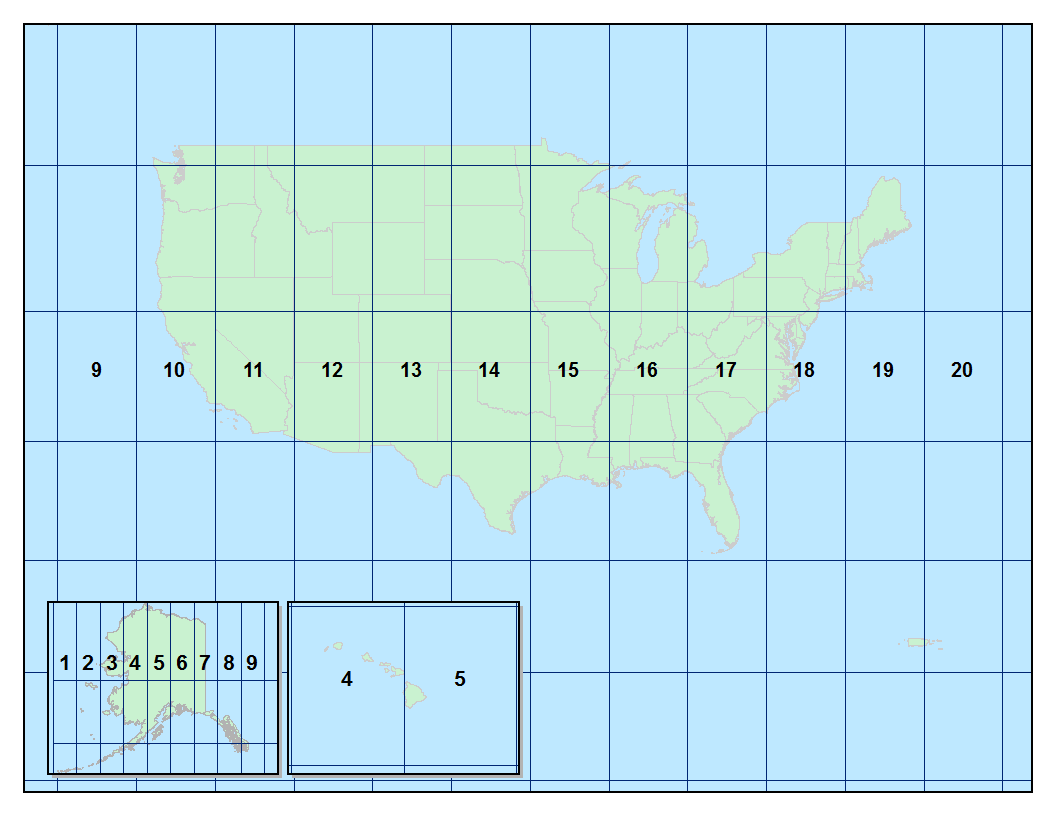
\includegraphics[scale = .35]{figures/UTMZoneMap2014.png}
    \caption{Index map of UTM zones}
    \label{fig: UMT zones}
\end{figure}

The initial selected zone, was zone 10. This zone represents the west coast of the United States, as it is shown in Figure ~\ref{fig: UMT zones}.
The chosen area, represents data whose longitude is from -120 to -126 and latitude is from 30 to 50, from a considerable amount of ships.

%http://www.marinecadastre.gov/ais/

\section{AIS Data}
 With the recent introduction of AIS in the Maritime domain the volume of vessel positional data as exponentially increased, a detailed description of this data, is found in section ~\ref{subsection: chp2_AIS}.

\begin{table}[H]
\centering
{\small
\begin{tabular}{lrrrrrl}
\toprule
{} &       MMSI &           X &          Y &   SOG &        COG &                Time \\
\midrule
0 &  636081210 & -125.993218 &  48.355773 &  14.3 &  73.300003 & 2014-02-27 13:33:02 \\
1 &  636081210 & -125.985303 &  48.357340 &  14.5 &  73.800003 & 2014-02-27 13:34:23 \\
2 &  636081210 & -125.979437 &  48.358500 &  14.6 &  73.099998 & 2014-02-27 13:35:23 \\
3 &  636081210 & -125.973353 &  48.359692 &  14.7 &  73.000000 & 2014-02-27 13:36:25 \\
4 &  636081210 & -125.965440 &  48.361318 &  15.0 &  73.000000 & 2014-02-27 13:37:46 \\
5 &  636081210 & -125.956733 &  48.363067 &  15.3 &  73.900002 & 2014-02-27 13:39:11 \\
6 &  636081210 & -125.950430 &  48.364153 &  15.7 &  76.099998 & 2014-02-27 13:40:11 \\
7 &  636081210 & -125.944108 &  48.365310 &  15.7 &  74.000000 & 2014-02-27 13:41:10 \\
8 &  636081210 & -125.937763 &  48.366510 &  15.9 &  73.900002 & 2014-02-27 13:42:12 \\
9 &  636081210 & -125.931385 &  48.367660 &  15.9 &  75.000000 & 2014-02-27 13:43:11 \\
\bottomrule
\end{tabular} }
\caption{Example of AIS data transmitted by Vessel, MMSI: 636081210}
\label{Table: TableAIS1}
\end{table}


\section{Route Representation}
Representing the data of a Vessel trajectory, can become a difficulty in the Maritime domain. There are a vast number of techniques described in the literature.

A effective way to represent a trajectory in the Maritime domain, is to look to the trajectory as a whole, this is, as vessel are obliged to broadcast their AIS information in a semi-continuous rates; knowing that each AIS broadcast message represent the instantaneous kinematic information from a single vessel, aggregating this information over time will represent a vessel trajectory. Therefore, knowing the MMSI of a vessel, a trajectory can be considered as the set of AIS messages broadcast, by that vessel, identified by the MMSI.


Thus, a possible definition for a vessel trajectory is a, set of multidimensional-points represented as:
\[TR_{MMSI} = p1, p2, p3, p4, \cdots , pn\]

Where each multidimensional point $p$ is defined as:
\[p = [t, x, y, SoG, CoG]\]


%\todo[inline]{ TODO SE FALTAR DADAS A INTERPOLAÇAO REALIZADA}


%for the Representation of MMSI as a track initially, then the assumption... interpolation of missing SOG and COG values. The use of Haversine formula, justify with as vessel motion is linear and no sudden speed exchanges or route exchanges tend to occur in secounds in the marite traffic, so this .

\section{MARISA Requirements}
